\documentclass[12pt,a4]{article}
\usepackage[margin=1in]{geometry} 
\usepackage{amsmath}
\usepackage{tcolorbox}
\usepackage{amssymb}
\usepackage{amsthm}
\usepackage{lastpage}
\usepackage{graphicx}
\usepackage{subfigure}
\usepackage{booktabs}
\usepackage{fancyhdr}
\usepackage{enumitem}
\usepackage{accents}
\pagestyle{fancy}
\usepackage{booktabs}
\setlength{\headheight}{40pt}
\usepackage[colorlinks=true,bookmarks=true]{hyperref}

\newenvironment{solution}
  {\renewcommand\qedsymbol{$\blacksquare$}
  \begin{proof}[Solution]}
  {\end{proof}}
\renewcommand\qedsymbol{$\blacksquare$}

\newcommand{\ubar}[1]{\underaccent{\bar}{#1}}

\begin{document}

\lhead{Guo Yiming \\PHY2009481} 
\rhead{BSC128 \\Numerical Method \\ Assignment 1} 
\cfoot{\thepage\ of \pageref*{LastPage}}
\rfoot{Code Repo: \href{https://github.com/yimingio/Lecture_Numerical_Method/tree/main/Assignment_1}{Github}}





\chead{Question 1} 

\begin{tcolorbox}
\textbf{Question 1} The forward-difference formula can be expressed as:
$$
f^{\prime}\left(x_{0}\right)=\frac{1}{h}\left[f\left(x_{0}+h\right)-f\left(x_{0}\right)\right]-\frac{h}{2} f^{\prime \prime}\left(x_{0}\right)-\frac{h^{2}}{6} f^{\prime \prime}\left(x_{0}\right)+O\left(h^{3}\right)
$$
Use extrapolation to derive an $O\left(h^{3}\right)$ formula for $f^{\prime}\left(x_{0}\right)$.
\end{tcolorbox}

\begin{solution}\ \\
Here we have that:


\begin{equation}
	f^{\prime}\left(x_{0}\right)=\frac{1}{h}\left(f\left(x_{0}+h\right)-f\left(x_{0}\right)\right)-\frac{h}{2} f^{\prime \prime}\left(x_{0}\right)-\frac{h^{2}}{6} f^{\prime \prime \prime}\left(x_{0}\right)+O\left(h^{3}\right) \label{Q1_1}
\end{equation}



Here we replace $h$ with $2h$


\begin{equation}
f^{\prime}\left(x_{0}\right)=\frac{1}{2 h}\left(f\left(x_{0}+2 h\right)-f\left(x_{0}\right)\right)-h f^{\prime \prime}\left(x_{0}\right)-\frac{4 h^{2}}{6} f^{\prime \prime \prime}\left(x_{0}\right) +O\left(h^{3}\right) \label{Q1_2}
\end{equation} 

Then we multiply \ref{Q1_1} with 2 and subtract the \ref{Q1_2}:


\begin{equation}
\begin{aligned}
&f^{\prime}\left(x_{0}\right)=\frac{2}{h}\left(f\left(x_{0}+h\right)-f\left(x_{0}\right)\right)-\frac{1}{2 h}\left(f\left(x_{0}+2 h\right)-f\left(x_{0}\right)\right)-\frac{h^{2}}{3} f^{\prime \prime \prime}\left(x_{0}\right)+\frac{2 h^{2}}{3} f^{\prime \prime \prime}\left(x_{0}\right)+O\left(h^{3}\right) \\
& \label{Q1_3}
\end{aligned}
\end{equation}



Next we replace the h with 2h in \ref{Q1_3}:


\begin{equation}
f^{\prime}\left(x_{0}\right)=\frac{1}{h}\left(f\left(x_{0}+2 h\right)-f\left(x_{0}\right)\right)-\frac{1}{4 h}\left(f\left(x_{0}+4 h\right)-f\left(x_{0}\right)\right)+\frac{4 h^{2}}{3} f^{\prime \prime \prime}\left(x_{0}\right)+O\left(h^{3}\right) \label{Q1_4}
\end{equation}

Then we multiply the \ref{Q1_3} with 4 and substract \ref{Q1_4}:


\begin{equation}
\begin{aligned}
3 f^{\prime}\left(x_{0}\right) &=\frac{8}{h}\left(f\left(x_{0}+h\right)-f\left(x_{0}\right)\right)-\frac{2}{h}\left(f\left(x_{0}+2 h\right)-f\left(x_{0}\right)\right)+\frac{4 h^{2}}{3} f^{\prime \prime}\left(x_{0}\right) \\
&-\frac{1}{h}\left(f\left(x_{0}+2 h\right)-f\left(x_{0}\right)\right)+\frac{1}{4 h}\left(f\left(x_{0}+4 h\right)-f\left(x_{0}\right)\right)-\frac{4 h^{2}}{3} f^{\prime \prime}\left(x_{0}\right)+O\left(h^{3}\right)
\end{aligned}
\end{equation}

And we can summarize that:


\begin{equation}
f^{\prime}\left(x_{0}\right)=\frac{1}{12 h}\left(f\left(x_{0}+4 h\right)-12 f(x_0+2 h)+32 f\left(x_{0}+h\right)-21 f\left(x_{0}\right)\right)+O\left(h^{3}\right)
\end{equation}






\end{solution}




\chead{Question 2} 

\begin{tcolorbox}
\textbf{Question 2} Determine the values of $n$ and $h$ required to approximate $\int_{0}^{2} x^{2} \sin (-x) d x$ to within $10^{-6}$ using the Composite Trapezoid Rule, Composite Midpoint Rule and Composite Simpson's Rule respectively.


Hint: You do not need to solve the numerical integration.
\end{tcolorbox}

\begin{solution}\ \\


Here we start with the Composite Trapezoid Rule, we recall that:
\begin{equation}
	\int_{a}^{b} f(x) d x=\frac{h}{2}\left[f(a)+2 \sum_{j=1}^{n-1} f\left(x_{j}\right)+f(b)\right]-\frac{b-a}{12} h^{2} f^{\prime \prime}(\mu)
\end{equation}


Here we have the error term as $\frac{b-a}{12} h^{2} f^{\prime \prime}(\mu)$, and then we find that maximum of of the error turn, first find the $|f''_{max}|$


 \begin{equation}
f(x)=x^{2} \sin (-x)
\end{equation}


\begin{equation}
f^{\prime}(x)=2 x \sin (-x)-x^{2} \cos (-x)
\end{equation}


\begin{equation}
f^{\prime \prime}(x) =\left(x^{2}-2\right) \sin (x)-4 x \cos (x)
\end{equation}

Here we try to find the absolute value of second derivative:


\begin{equation}
\begin{aligned}
\left|f^{\prime \prime}(x)\right| &=\left|\left(x^{2}-2\right) \sin (x)-4 x \cos (x)\right| \\
&\leq | \left( x^{2}-2\right) \sin (x)|+| 4 x \cos (x) | \\
& \leq\left|x^{2}-2\right|+|4 x| \leq\left|(2)^{2}-2\right|+|4 \cdot 2|=10
\end{aligned}		\label{f''}
\end{equation}



Therefore we can derive the error term's maximum


\begin{equation*}
\frac{b-a}{12} h^{2} f^{\prime \prime}(\mu) \leq \frac{2-0}{12} h^{2} \cdot 10 \leq 10^{-6}
\end{equation*}


And it turn out that:


$$
h \leq 7.7460 \times 10^{-4}
$$


And we can have the $n$ that:


$$
n \geq \frac{b-a}{h}=2582
$$







\dotfill


Next we find the Composite Midpoint Rule


\begin{equation}
\int_{a}^{b} f(x) d x=2 h \sum_{j=0}^{n / 2}+\frac{b-a}{6} h^{2} f^{\prime \prime}(\mu)
\end{equation}


And we have the second derivative same with the previous one:


\begin{equation}
f^{\prime \prime}(x)=\left(x^{2}-2\right) \sin (x)-4 x \cos (x)
\end{equation}

This part is similar with the part in \ref{f''}, and we can caculate the error term here:


$$
\frac{b-a}{b} h^{2} f^{\prime \prime}(\mu)\leq \frac{2-0}{6} h^{2} \cdot 10 \leq 10^{-6}
$$


$$
h \leq 5.477 \times 10^{-4}
$$


And we can turn out that:
$$
n \geq \frac{b-a}{h}=3652
$$





\dotfill




Next we find the Composite Simpson Rule

\begin{equation*}
	\int_{a}^{b} f(x) d x=\frac{h}{3}\left[f(a)+2 \sum_{j=1}^{(n / 2)-1} f\left(x_{2 j}\right)+4 \sum_{j=1}^{n / 2} f\left(x_{2 j-1}\right)+f(b)\right]-\frac{b-a}{180} h^{4} f^{(4)}(\mu)
\end{equation*}


Here the error term is $\frac{b-a}{180} h^{4} f^{(4)}(\mu)$, then we first find the fourth derivative:


\begin{equation*}
\begin{aligned}
f^{\prime \prime}(x)&=\left(x^{2}-2\right) \sin (x)-4 x \cos (x) \\
f^{\prime \prime \prime}(x)&=\left(x^{2}-6\right) \cos (x)+6 x \sin (x) \\
f^{(4)}(x)&=8 x \cos (x)-\left(x^{2}-12\right) \sin (x)
\end{aligned}
\end{equation*}


Next determine the maximum of the fourth derivative:


\begin{equation*}
\begin{aligned}
\left|f^{(4)}(x)\right| &=\left|8 x \cos (x)-\left(x^{2}-12\right) \sin (x)\right| \\
& \leq|8 x \cos (x)|+\mid\left(x^{2}-127 \sin (x) \mid\right.\\
& \leq|8 x|+\left|x^{2}-12\right|=8 x+12-x^{2} \\
&=-(x-4)^{2}+28 \leq 24
\end{aligned}
\end{equation*}


And the error term could be transform into below form:


\begin{equation}
\begin{aligned}
	\frac{2-0}{180} h^{4} \cdot 24 &\leq 10^{-6}\\
	h & \leq 4.401 \times 10^{-2}
\end{aligned}
\end{equation}

And we can turn out that:


\begin{equation}
n \geq \frac{b-a}{h}=4 6
\end{equation}



















\end{solution}




















\chead{Question 3} 


\begin{tcolorbox}
\textbf{Question 3} 

Given a function, $f(t)=\sqrt{t}$


a) Apply the Romberg Integration to find $R_{3,3}$ for the integral $\int_{1}^{4} f(t) d t$.


b) Apply the Composite Simpson's Rule to approximate $\int_{1}^{4} f(t) d t$ using eight intervals.


c) Comment on your results in (a) and (b).

\end{tcolorbox}

\begin{solution}\ \\

(a)
\begin{equation}
\begin{aligned}
&R_{1,1}=\frac{4-1}{2}(\sqrt{1}+\sqrt{4})=\frac{9}{2}=4.500 \\
&R_{2,1}=\frac{4-1}{4}\left(\sqrt{1.1}+2 \sqrt{\frac{1+4}{2}}+\sqrt{4}\right)=\frac{3}{4}(3+\sqrt{10})=4.622 \\
&R_{2,2}=R_{2,1}+\frac{1}{3}\left(R_{2,1}-R_{1,1}\right)=4.663 \\
&R_{3,1}=\frac{4-1}{8}\left(\sqrt{1}+2 \sqrt{\frac{7}{4}}+2 \sqrt{\frac{5}{2}}+2 \sqrt{\frac{13}{4}}+\sqrt{4}\right)=\frac{3}{8}(3+\sqrt{7}+\sqrt{10}+\sqrt{13})=4.655 \\
&R_{3,2}=R_{3,1}+\frac{1}{3}\left(R_{3,1}-R_{2,1}\right)=4.666 \\
&R_{3,3}=R_{3,2}+\frac{1}{4^{2}-1}\left(R_{3,2}-R_{2,2}\right)=4.666
\end{aligned}
\end{equation}



And we can plot the graph as:


\begin{equation*}
\begin{array}{lll}
\hline
4.500 & & \\
4.622 & 4.663 & \\
4.655 & 4.666 \quad 4.666 \\
\hline
\end{array}
\end{equation*}

\dotfill



(b) Here $n=8$, $h=\frac{4-1}{8}$, $x_{j}=1+\frac{3}{8} j$:


\begin{equation}
\begin{aligned}
\int_{1}^{4} f(t) d t &=\frac{1}{3} \frac{3}{8}\left(f(1)+2\left(f\left(x_{2}\right)+f\left(x_{4}\right)+f\left(x_{6}\right)\right)+4\left(f\left(x_{1}\right)+f\left(x_{3}\right)+f\left(x_{5}\right)+f\left(x_{7}\right)+f(49)\right)\right.\\
&=\frac{1}{8}\left(f(1)+2\left(f\left(\frac{7}{4}\right)+f\left(\frac{5}{2}\right)+f\left(\frac{13}{4}\right)\right)+ \right.\\
&\quad \left. 4\left(f\left(\frac{11}{8}\right)+f\left(\frac{17}{8}\right)+f\left(\frac{23}{8}\right)+f\left(\frac{29}{8}\right)\right)+f(4)\right)\\
&=\frac{1}{8}(3+\sqrt{7}+\sqrt{10}+\sqrt{13}+\sqrt{22}+\sqrt{34}+\sqrt{46}+\sqrt{58}) \\
&=4.667
\end{aligned}
\end{equation}

\dotfill

(c)Here we can first calculate the exact value of the solution


$$
\begin{aligned}
\int_{1}^{4} f(t) d t &=\int_{1}^{4} t^{\frac{1}{2}} d t=\left(\frac{2}{3} t^{\frac{3}{2}}\right)_{1}^{4}=\frac{2}{3} \cdot(8-1)=\frac{14}{3}=4 \frac{2}{3} \\
&=4.666 \cdots
\end{aligned}
$$

And we can find that both method give a very close answer with the exact value. And Composite Simpson Law seems to be closer to the exact result.However due to the rounding off 4 digits, we can not see what exact is the error for this 2 methods, 







\end{solution}




\chead{Question 4} 

\begin{tcolorbox}
\textbf{Question 4} 







\end{tcolorbox}

\begin{solution}\ \\











\end{solution}

\chead{Question 5} 




\begin{tcolorbox}
\textbf{Question 5} 
Given $f(x)=2-x^{2} \sin (x)$ has a solution in the interval $[-1,2]$.
\begin{enumerate}[label=(\alph*)]
	\item Sketch the graph for $f(x)$ on interval $[-10,10]$
	\item Apply five steps of Newton's Method with initial guess $x_{0}=-1$ to attempt to find this root.
	\item Apply five steps of Newton's Method with initial guess $x_{0}=2$ to attempt to find this root.
	\item Compare the results of (b) and (c), explain what happens.
\end{enumerate}

\end{tcolorbox}

\begin{solution}\ \\


\begin{enumerate}[label=(\alph*)]

\item
The Diagram generated by MatLab (\ref{Q5_a_1})\\
\begin{figure}[htb]
	\centering %图片居中
  	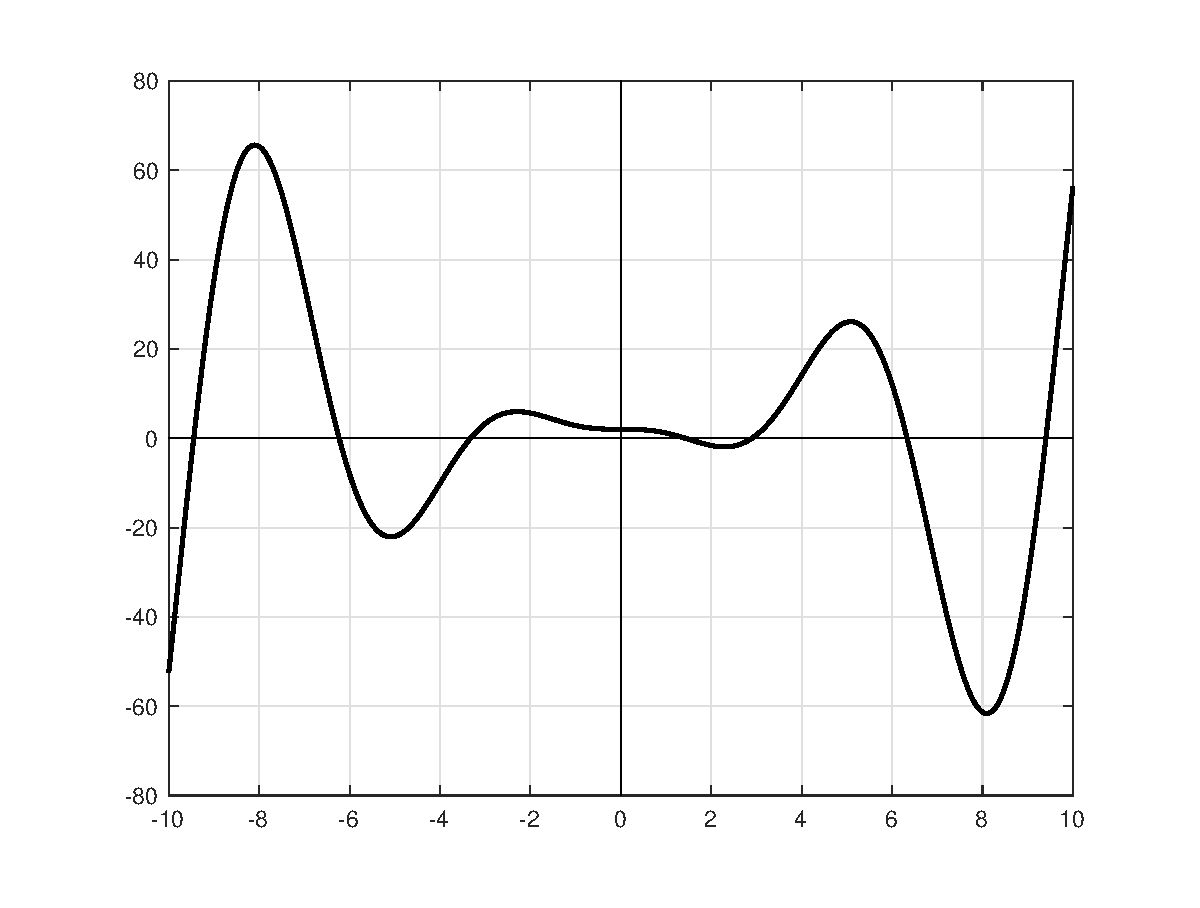
\includegraphics[width=0.7\textwidth]{fig/Q5_plot.eps}
  	\caption{(a) $f(x)=2-x^2 \sin(x)$} \label{Q5_a_1}
\end{figure}


\item Here first find the iteration method.\\

\begin{equation}
	x_{i+1}=x_{i}-\frac{f\left(x_{i}\right)}{f^{\prime}\left(x_{i}\right)} \label{Q5_iteration}
\end{equation}


Here the function is given that

\begin{equation}
	f(x)=2-x^2\sin (x) \label{Q5_equation}
\end{equation}

\begin{equation}
	f'(x)=-2x \sin(x) - x^2 \cos(x) \label{Q5_equation_derivative}
\end{equation}

Therefore input (\ref{Q5_equation}) and (\ref{Q5_equation_derivative}) into (\ref{Q5_iteration}),the function is given that:


\begin{equation}
	x_{i+1} =x_{i}-\frac{2-x_i^2\sin (x_i)}{-2x_i \sin(x_i) - x_i^2 \cos(x_i)} 
\end{equation}
	
	
In this section we set the initial guess, $x_0=-1$:



$$
x_{1} =x_{0}-\frac{2-x_0^2\sin (x_0)}{-2x_0 \sin(x_0) - x_0^2 \cos(x_0)}=0.2781
$$ 

$$
x_{2} =x_{1}-\frac{2-x_1^2\sin (x_1)}{-2x_1 \sin(x_1) - x_1^2 \cos(x_1)}=8.994
$$ 


$$
x_{3} =x_{2}-\frac{2-x_2^2\sin (x_2)}{-2x_2 \sin(x_2) - x_2^2 \cos(x_2)}=9.475
$$ 

$$
x_{4} =x_{3}-\frac{2-x_3^2\sin (x_3)}{-2x_3 \sin(x_3) - x_3^2 \cos(x_3)}=9.403
$$ 

$$
x_{5} =x_{4}-\frac{2-x_4^2\sin (x_4)}{-2x_4 \sin(x_4) - x_4^2 \cos(x_4)}=9.402
$$ 


\item

In this section we set the initial guess, $x_0=2$:

$$
x_{1} =x_{0}-\frac{2-x_0^2\sin (x_0)}{-2x_0 \sin(x_0) - x_0^2 \cos(x_0)}=1.170
$$ 

$$
x_{2} =x_{1}-\frac{2-x_1^2\sin (x_1)}{-2x_1 \sin(x_1) - x_1^2 \cos(x_1)}=1.445
$$ 


$$
x_{3} =x_{2}-\frac{2-x_2^2\sin (x_2)}{-2x_2 \sin(x_2) - x_2^2 \cos(x_2)}=1.422
$$ 

$$
x_{4} =x_{3}-\frac{2-x_3^2\sin (x_3)}{-2x_3 \sin(x_3) - x_3^2 \cos(x_3)}=1.422
$$ 

$$
x_{5} =x_{4}-\frac{2-x_4^2\sin (x_4)}{-2x_4 \sin(x_4) - x_4^2 \cos(x_4)}=1.422
$$ 


\item




Here we first plot the graph of the iteration point generated by 5(b) and 5(c), (\ref{Q5_d_1}):

\begin{figure}[htb]
\centering
\subfigure[5(b)]{
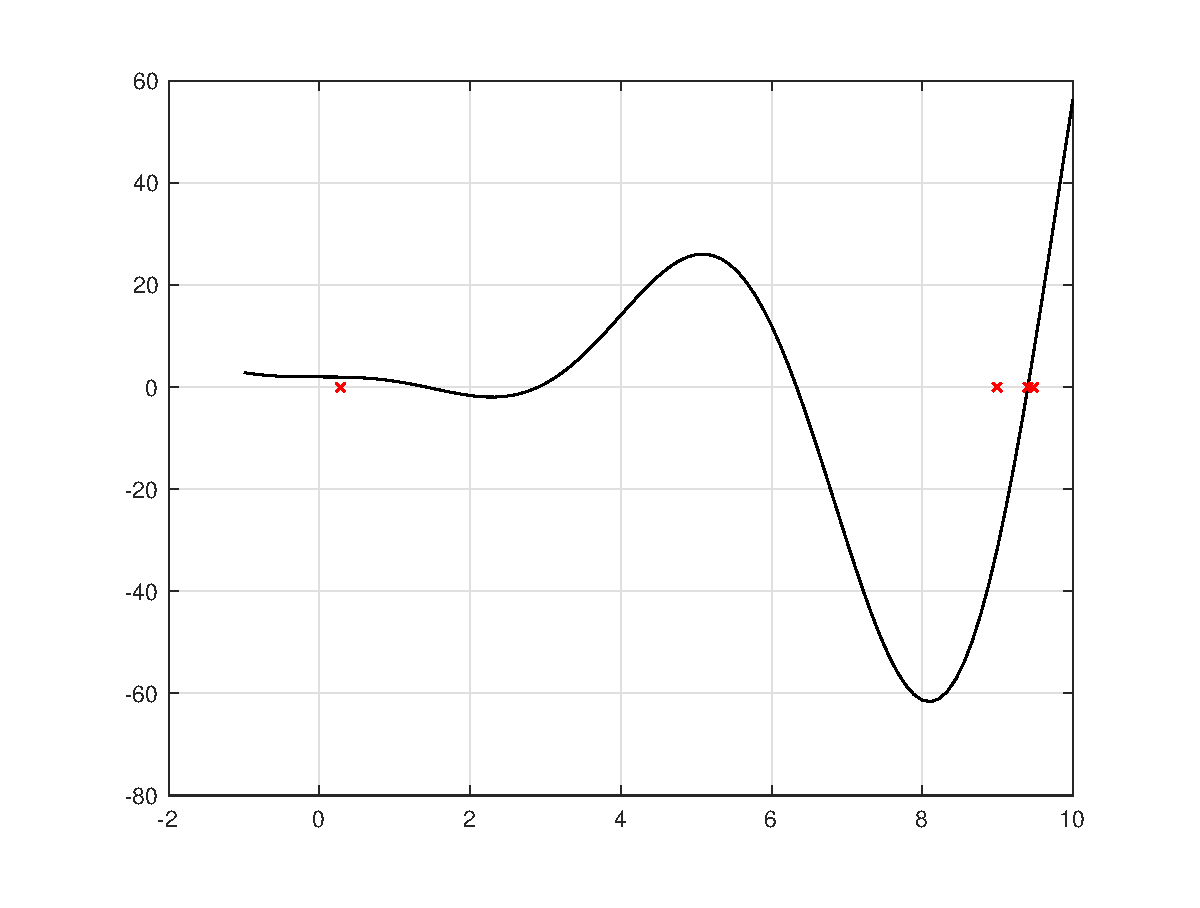
\includegraphics[width=7.5cm]{fig/Q5_d_1.eps}
%\caption{fig1}
}
\quad
\subfigure[5(c)]{
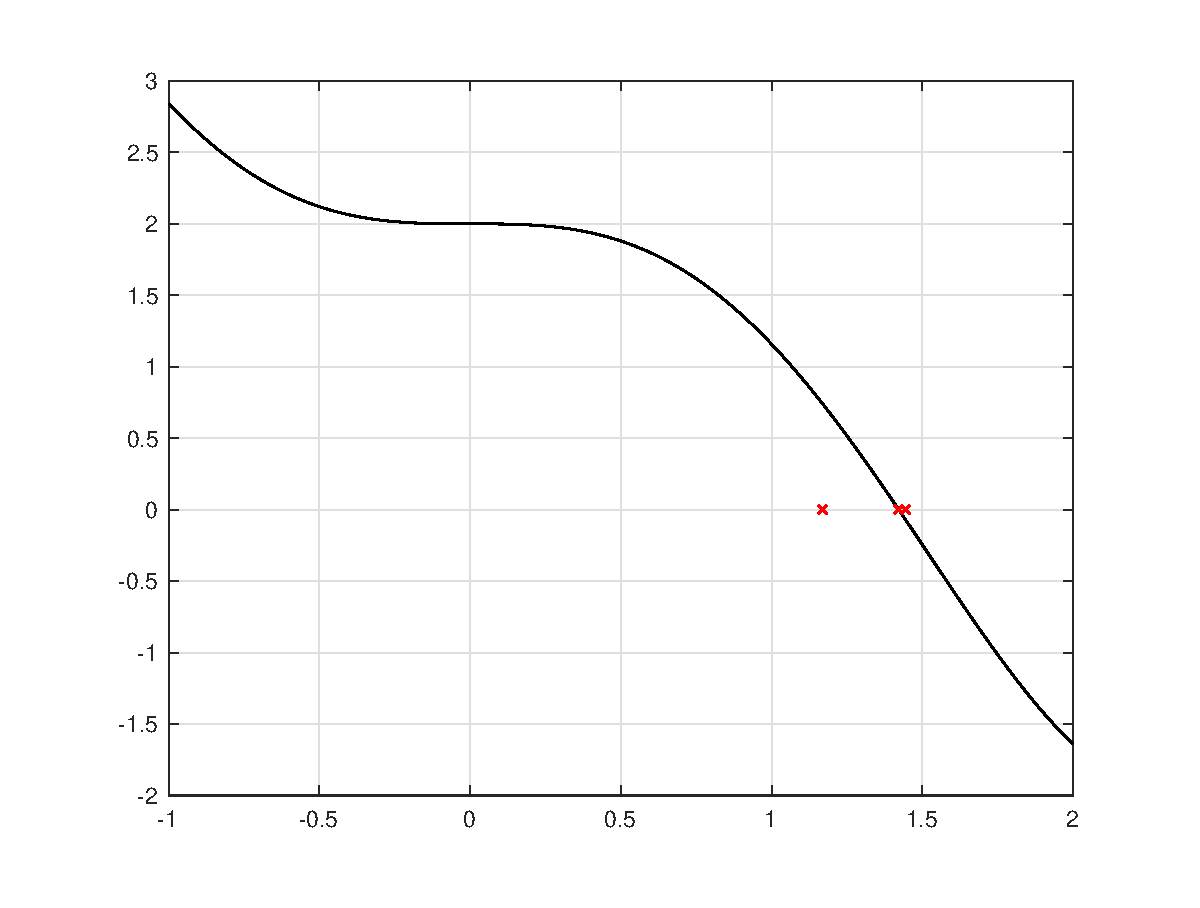
\includegraphics[width=7.5cm]{fig/Q5_d_2.eps}
}
\caption{Iteration Point of 5(b) and 5(c)}
\label{Q5_d_1}
\end{figure}



Therefore it is easy to find that in 5(b),the initial guess leads to the root jump to another region, out of the required range. Which is one of the drawback of the Newton's Method: In some cases where the function is oscillating and has a number of roots, one may choose an initial guess close to a root. However, the guesses may jump and converge to some other root.


Here we can plot the graph to illustrate the procedure of the root jumping in 5(b),(\ref{5_d_3}). Newton's Method could be described in figure that we choose one point and found the tangent line on $f(x)$, the focus of the tangent and X axis will be the result and the initial value of the next iteration. Here we hope the focus point can be closer to the root we want. 



\begin{figure}[htb] %H为当前位置,!htb为忽略美学标准,htbp为浮动图形
\centering %图片居中
\includegraphics[width=0.6\textwidth]{fig/Q5_d_3.eps} %插入图片,[]中设置图片大小,{}中是图片文件名
\caption{The procedure of the root jumping in 5(b)} %最终文档中希望显示的图片标题
\label{5_d_3} %用于文内引用的标签
\end{figure}







However in 5(b), when the second times of the iteration leads to an abnormal focus with the x axis. This is because in the local region, the slope is too small and turn to be flat (\ref{Q5_d_4}), which leads the focus locate in second iteration far from the required region, at $8.994375358445748$, and then the further iteration leads to converge to another root around $9.4$.


In 5(c) we start at $x_0=2$, here by plotting the graph of the derivative, we can find that the slope is enough to let the result converge to the root without jumping. (\ref{Q5_d_4})


\begin{figure}
\centering
\subfigure[5(b)]{
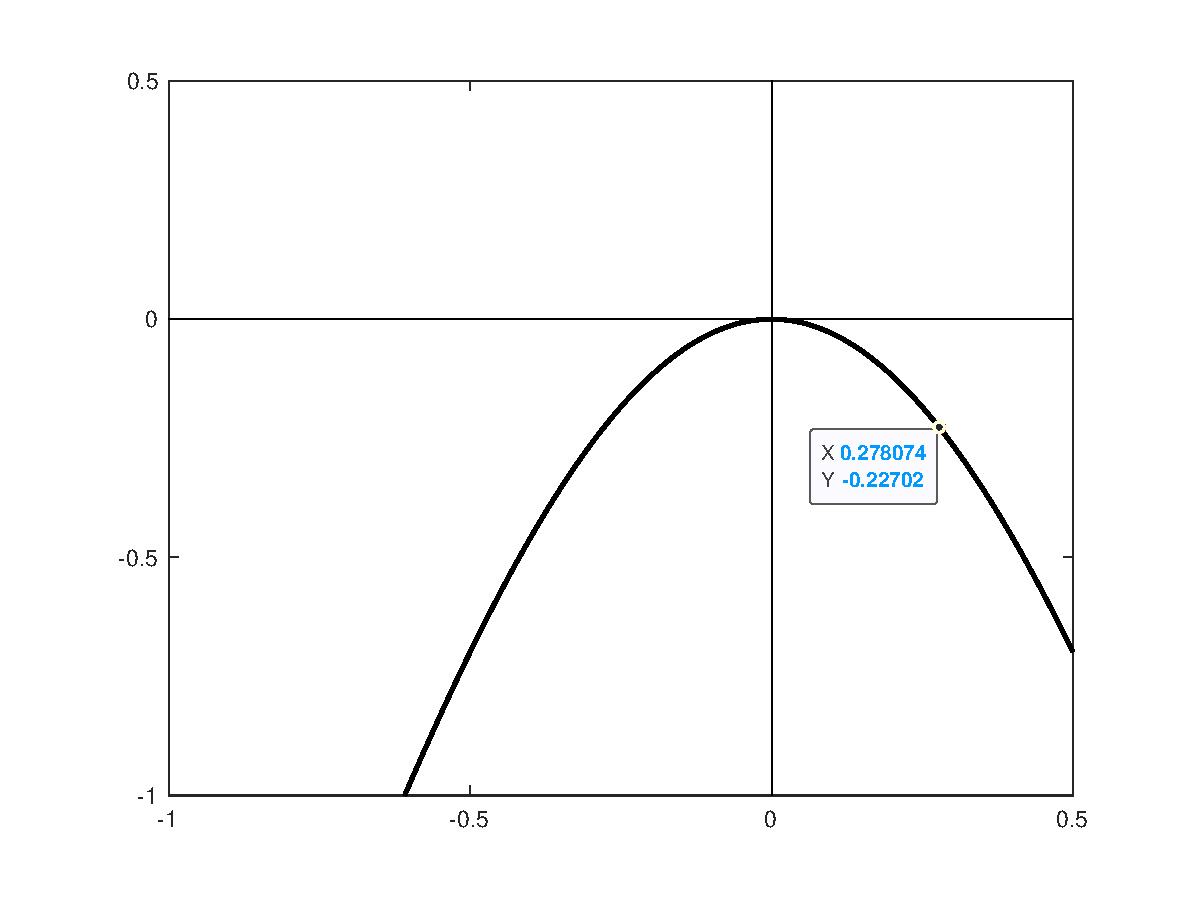
\includegraphics[width=7.5cm]{fig/Q5_d_4.eps}

}
\quad
\subfigure[5(c)]{
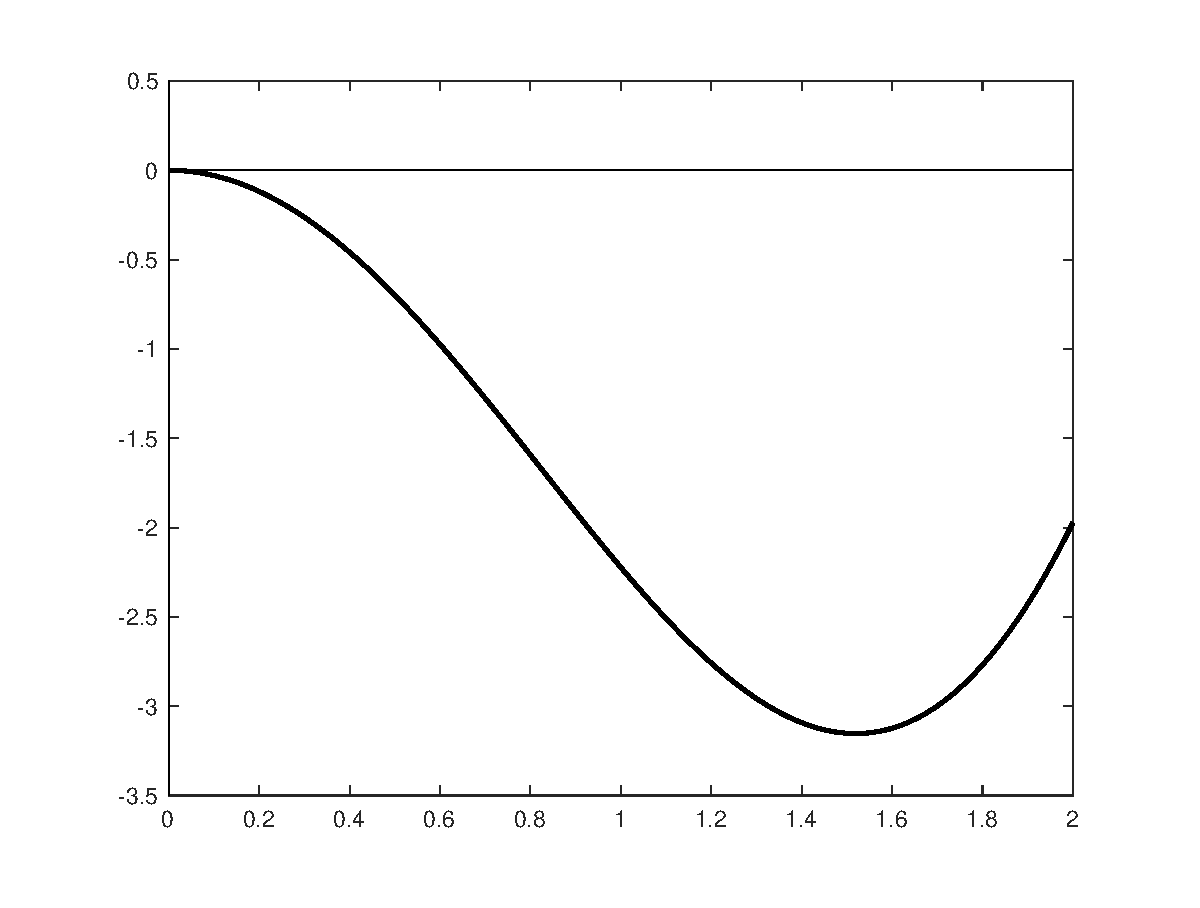
\includegraphics[width=7.5cm]{fig/Q5_d_5.eps}

}

\caption{Function first derivative (slope) diagram}
\label{Q5_d_4}
\end{figure}





To prevent the Root jumping problem when applying the Newton's Method, several tips could be applied to overcome:
\begin{enumerate}
	\item When the function is oscillating or have many roots, The Method of False Position may be a better choice. It has strong stability, but it lags behind in efficiency.
	\item Before iteration, check whether there is a phenomenon that the slope approaches zero near the selected initial point, which will lead to serious deviation of the iterative results in Newton method.
	\item  Choose the point closer to the unknown root as the initial point, which will improve the stability and efficiency of the model to a certain extent.
\end{enumerate}

















	
	
\end{enumerate}


\end{solution}








\end{document}
